Um die Funktionsweise beider Algorithmen zu belegen wurden beide Methoden einerseits auf ihre Robsutheit und andrerseites auf ihre Performance getestet. Im folgenden Kapitel wird zunächst das zum Testen verwendete Setup beschrieben. Anschliessend erfolgt die Auswertung der erlangten Testergebnisse. Zuletzt werden weitere Tests durchgeführt welche das System kritischen Situationen testen soll.

% ---------------------- section -----------------------
\section{Testsetup}
\label{sec:aufbau}

Bei der Durchführung der Tests befinden sich die Kameras statisch im Raum. Die zu erkennenden Hindernisse werden innerhalb und ausserhalb der zu erkennenden Reichweite platziert, wobei die Ausrichtung der Hindernisse teils zufällig, teils bewusst an kritischen Positionen erfolgt, um ein reales Anwendungsszenarien passend zu simulieren. Ein aufgenommenes Testset besteht dabei aus beiden Bildern der Kamera, der normalisierten Disparity Map sowie eine komplette Pointcloud dieser um etwaige Fehler der Algorithmen leichter erkennen zu können, sowie den geloggten Pointclouds der Hinderniserkennung. Weiterhin werden diverse Parameter gespeichert, wie die Anzahl der erkannten Hinderniselemente, sowie deren Disparitäten.\\

\noindent
Der zu erkennende Bereich wurde auf $0,2$ bis $1,5$ Meter definiert. Dies entspricht einem Szenario in welchem das System auch aufgrund der hohen Framerate der Erkennung angewendet werden kann. Eine Erweiterung dessen auf beispielsweise $2.0$ Meter wurde nicht durchgeführt, da der Algorithmus auch bei großen Entfernungen robuste Werte in der Distanzberechnung liefert \cite{hilleralhallak}.
Das dabei erreichte Sichtfeld nach der Anwendug der ROI auf die Disparity Map (siehe \ref{sec:preprocessing}) beträgt $50^{\circ}$ auf horizontaler Achse und $38^{\circ}$ vertikal. Dies ist in Abbildung (REF) visualisiert.
	% TODO sichtfeld durch disparity map & vergleich zum ursprünglichen sichtfeld

\noindent
Ein aufgenommenes Testset besteht aus jeweils 12 Testbildern. Für jede Methode wurden drei verschiedene Hindernisgrößen getestet, groß, klein und winzige Hindernisse. Anhand dieser wird ausgewertet welche minimale, maximale sowie mittlere Disparität, und daraus resultierende Distanz erkannt wird.\\

\noindent
Weitere Tests beinhalten die Erkennung winziger Hindernisse unter Veränderung der \emph{SGBM} Parameter. Dabei wird unter anderem untersucht ob beispielsweise eine verringerte Blockgröße Einfluss auf die Erkennung kleiner Bereiche nimmt. Des Weiteren wird die Zeit für die Hinderniserkennung eines Frames untersucht um eine durchschnittliche Zeit für die Erkennung sowie die daraus resultierende Framerate zu ermitteln. Dies geschieht einerseits durch die Erkennung eines Hindernisses, welches sich über das gesamte Bild ausbreitet, andererseits für nur ein Teilelement jeder Erkennungsmethode (Subimage, Samplepoint).\\
Zudem wird geprüft inwiefern die Algorithmen mit Limitierungen des \emph{SGBM} umgehen können. Dazu zählen die Erkennung bei spiegelnden, reflektierenden und durchsichtigen Flächen, sowie die Erkennung schwach texturierter Hindernisse.\\

% kameras statisch im raum
% hindernisse innerhalb der zu erkennenden reichweite platziert
% ausrichtung der hinernisse zum teil zufällig
% teils bewusst an kritischen positionen platizert
% für jeden Frame werden Informationen geloggt wie anzahl der erkannten hindernisse sowie position der hindernisse im raum
% für jeden frame wird eine vollständige pointcloud berechnet um etwaige fehler zu erkennen
% verschiedene hindernisgrößen gross klein winzig
% jeweils 12 testbilder
% range auf 0.2 - 1.5 meter festgelegt --> real life szenario

% weitere tests:
	% erkennung von kleinen hindernissen mithilfe veränderter sgbm parameter
	% zeit die fuer die ausführung der detectObstacles funktion benötigt wird
	% können auch extreme situationen wie durchsichtige flächen erkannt werden?
		% spiegelnd
	% erkennung von wenig texturierten hindernissen
	% 

% ---------------------- section -----------------------
\section{Evaluierung Subimage Detection}
\label{sec:evaluierung_subimage}

    \subsection{Robustheit}
    \label{subsec:subimage_robustheit}
    
    % allgemein hindernisse beschreiben
    	% welche fläche repräsentiert jedes hinderniss
    	% was ist daran gut / scchelcht vielleicht
    
	% hinsichtlich robustheit
	% beschriebene testsets werden ausgewertet
	% nach der Anzahl der erkannte hindernisse
	% den gespeicherten weltdistanzen
	% den daraus resultierentden median werten der distanz
		% berechnet und gemessen
	% werden Hindernisse erkannt
	% wie hoch ist der drift zwischen den einzelnen sets
	% vielleicht standartabweichung betrachten
	% für jedes set einzeln
	% woher kommen die drifts 
		% (person im bild bei der bildaufnahme
		% hindernisse im winkel gehalten --> geneigt
	% trotzallem wurde jedes hindernis erkannt
	% abweichung entsteht einerseits durch besagten drift durch beschriebene gruende
		    
\begin{figure}[h]
	\centering
	\begin{tabular}{m{7.0cm} m{7.0cm}}
	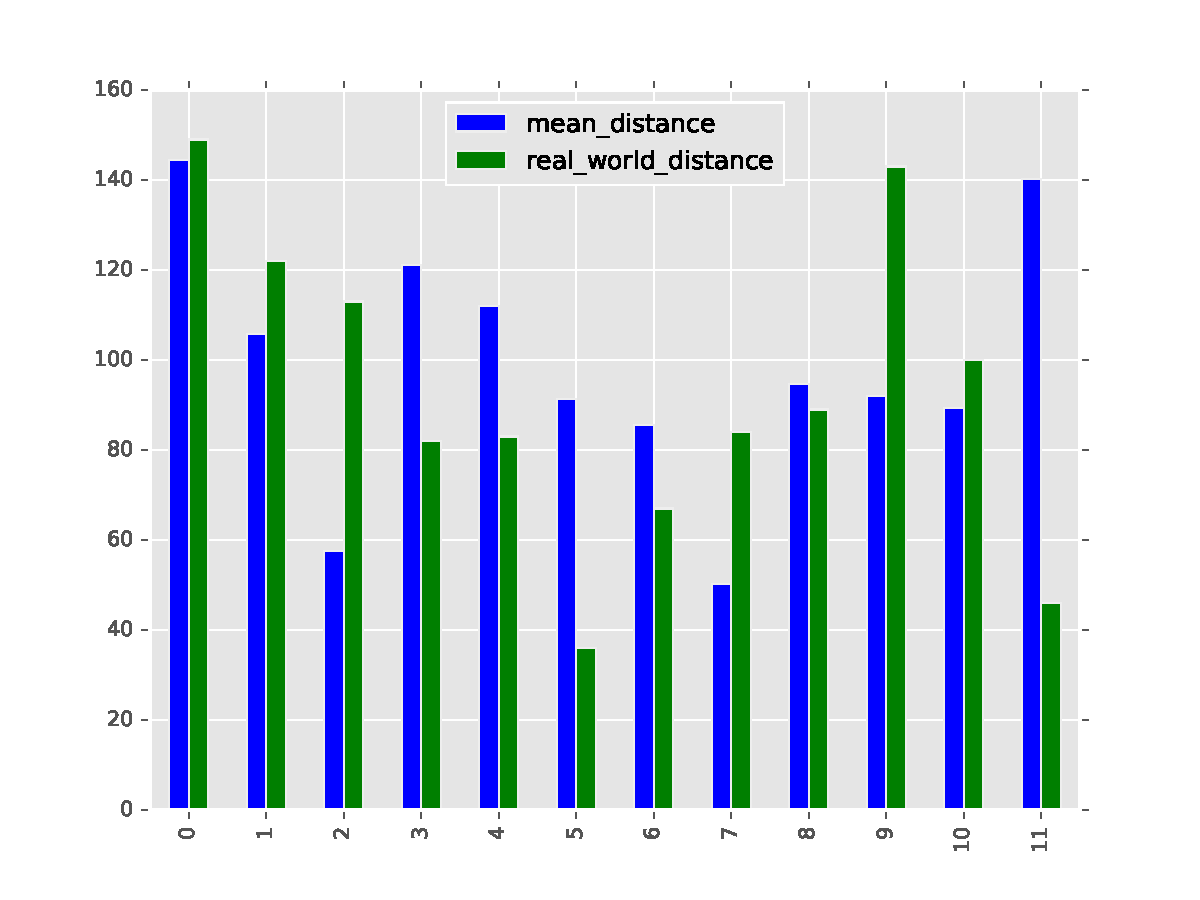
\includegraphics[width=7cm]{img/evaluation/big_bar}
	\centering \small (a)
	&
	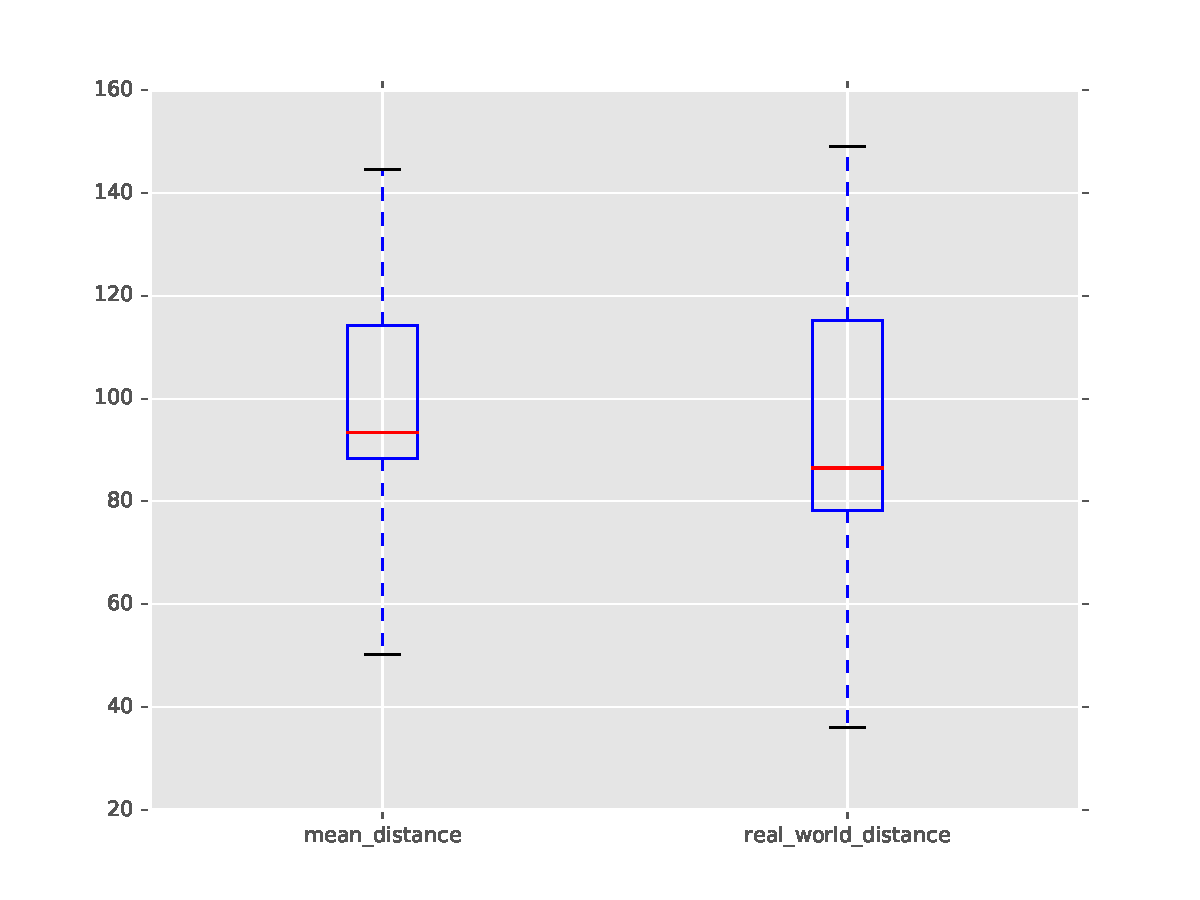
\includegraphics[width=7cm]{img/evaluation/big_box}
	\centering \small (b)
	\end{tabular}
    \caption{}
    \label{fig:eval_big}
\end{figure}

\begin{figure}[h]
	\centering
	\begin{tabular}{m{7.0cm} m{7.0cm}}
	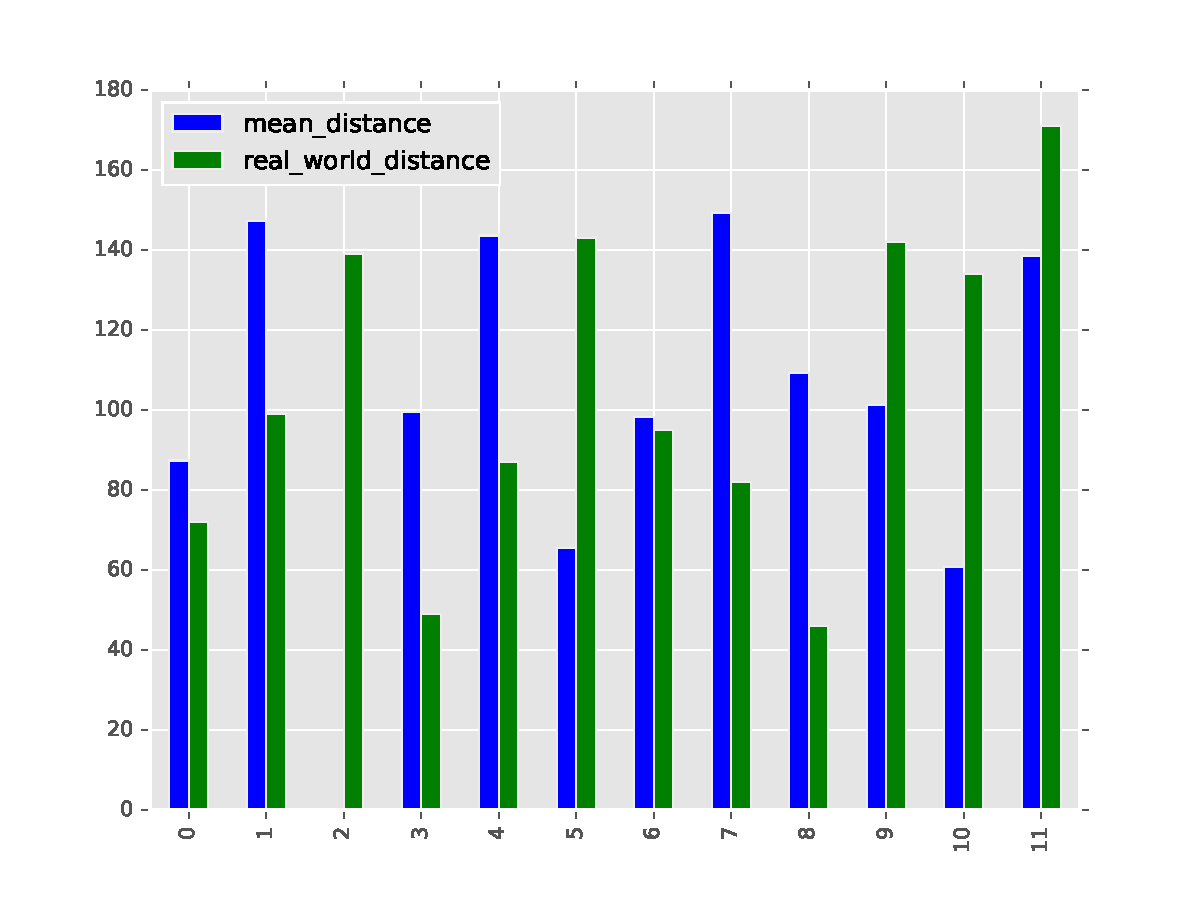
\includegraphics[width=7cm]{img/evaluation/medium_bar}
	\centering \small (a)
	&
	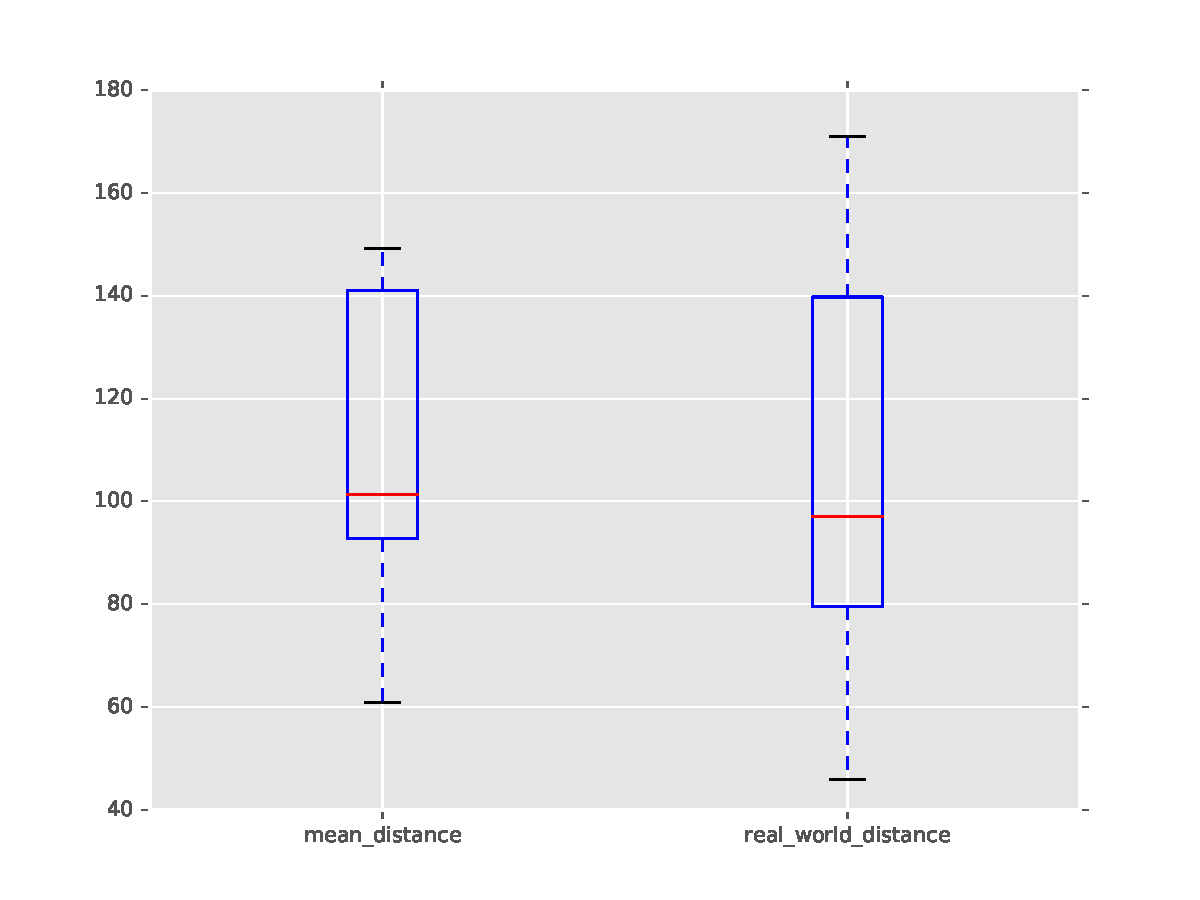
\includegraphics[width=7cm]{img/evaluation/medium_box}
	\centering \small (b)
	\end{tabular}
    \caption{}
    \label{fig:eval_medium}
\end{figure}

\begin{figure}[h]
	\centering
	\begin{tabular}{m{7.0cm} m{7.0cm}}
	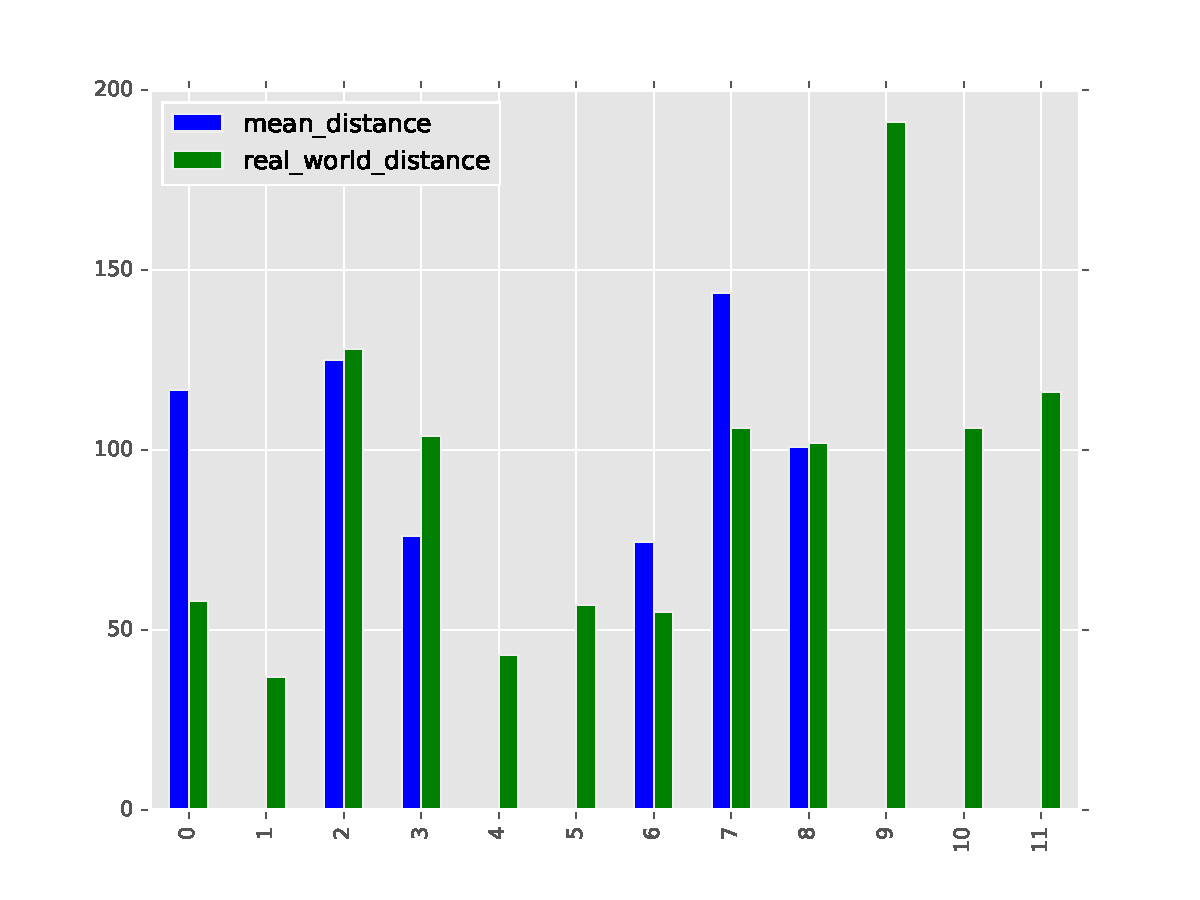
\includegraphics[width=7cm]{img/evaluation/tiny_bar}
	\centering \small (a)
	&
	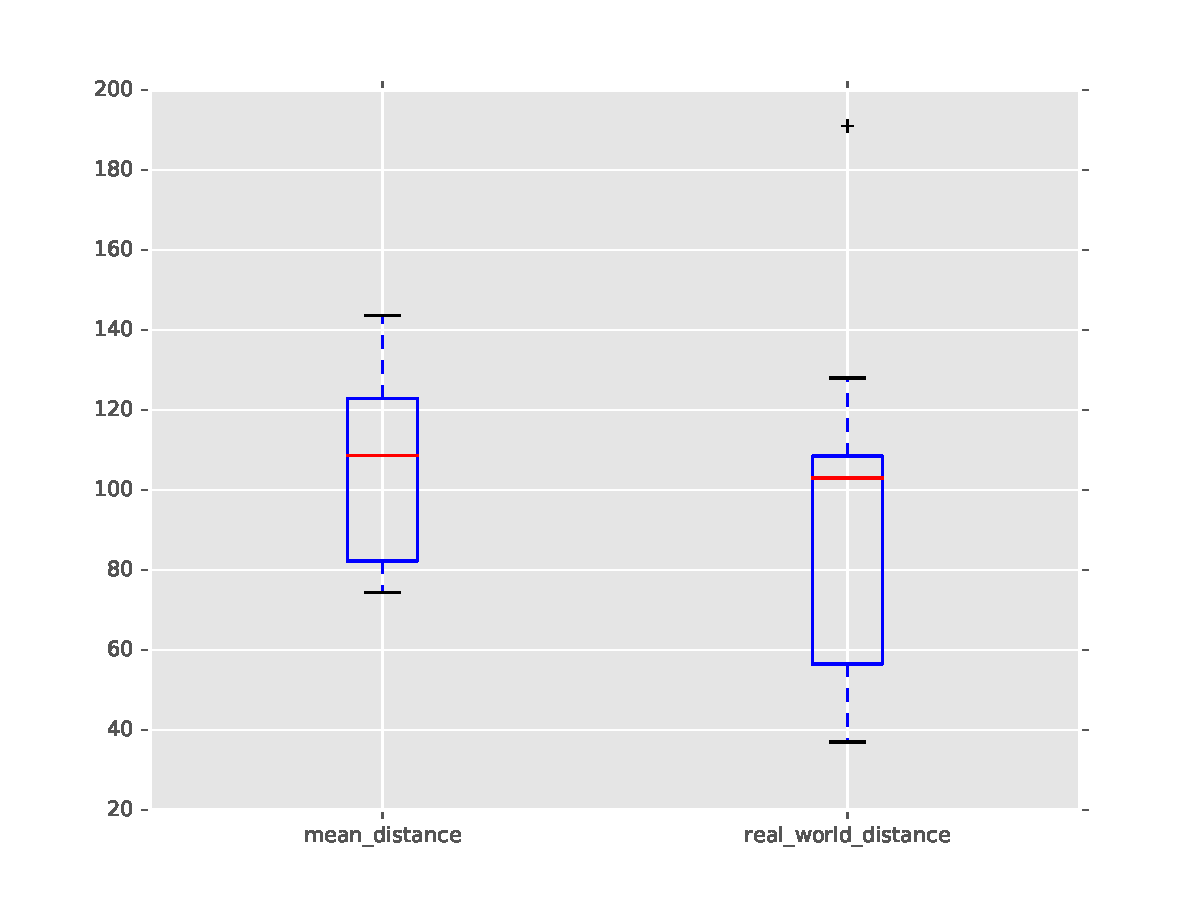
\includegraphics[width=7cm]{img/evaluation/tiny_box}
	\centering \small (b)
	\end{tabular}
    \caption{}
    \label{fig:eval_tiny}
\end{figure}

    \subsection{Performanz}
    \label{subsec:subimage_performanz}

% ---------------------- section -----------------------
\section{Evaluierung Samplepoint Detection}
\label{sec:evaluierung_samplepoint}

    \subsection{Robustheit}
    \label{subsec:samplepoint_robustheit}    

    \subsection{Performanz}
    \label{subsec:samplepoint_performanz}